\documentclass[11pt]{beamer} % Определяем тип документа как презентацию
% в квадратных скобках размер шрифта: 8pt, 9, 10, 11 (def), 12, 14, 17, 20.

% Общее:
\usetheme{CambridgeUS} % колонтитулы, углы, и другая красота
% Другие темы можно найти на https://latex-beamer.com/tutorials/beamer-themes/
\usecolortheme{seahorse} % но по факту мы почти все цвета сами задаем
% https://deic.uab.cat/~iblanes/beamer_gallery/index_by_color.html
\usefonttheme{professionalfonts}

\usepackage {mathtools} % красивая математика
\usepackage{amsmath,amsfonts,amssymb,amsthm,mathtools} % еще математика

\usepackage[
backend=biber,
style=numeric,
sorting=nty
]{biblatex} % для библиографии
\addbibresource{references.bib}
\usepackage{hyperref} % для ссылок
\usepackage{epigraph}
\usepackage{graphicx}

% Создаем цвета
\definecolor{darkredNES}{RGB}{115,15,15} % тёмно-красный
\definecolor{darkblueNES}{RGB}{20,20,100} % тёмно-синий
\definecolor{redNES}{RGB}{170,35,35} % красный посветлее
\definecolor{darkgreenNES}{RGB}{7,110,7} % тёмно-зеленый
\definecolor{alertredNES}{RGB}{125,25,25} % красный средний
% Однако в основном проще пользоваться стандартными цветами, подробнее тут:
% https://www.overleaf.com/learn/latex/Using_colours_in_LaTeX

\setbeamercolor*{palette primary}{bg=darkblueNES} %правые рамки
\setbeamercolor*{palette secondary}{bg=darkblueNES, fg = white} %центральные
\setbeamercolor*{palette tertiary}{bg=darkblueNES, fg = white} %левые

\setbeamercolor*{titlelike}{bg=darkblueNES} % названия слайдов
\setbeamercolor*{title}{bg=darkblueNES, fg = white} % титул и отделы
\setbeamercolor*{item}{fg=redNES} % для списков (например, в оглавлении)
\setbeamercolor*{caption name}{fg=darkblueNES} % названия картинок
\setbeamercolor{alerted text}{fg=alertredNES} % выделенка

\setbeamertemplate{blocks}[rounded, shadow=true]
\setbeamercolor{block title}{bg=darkblueNES, fg=white}
\setbeamercolor{block title alerted}{bg=alertredNES, fg=white}
\setbeamercolor{block title example}{bg=darkgreenNES, fg=white}

\setbeamercolor{bibliography entry author}{fg=black}
\setbeamercolor{bibliography entry title}{fg=black}
\setbeamercolor{bibliography entry note}{fg=darkblueNES}

\setbeamercolor{page number in head/foot}{fg=white}

% Для русского нам пригодится
\usepackage[english]{babel} % локализация и переносы
\usepackage{fontspec}
\usepackage[T2A]{fontenc} % кодировка
\usepackage[utf8]{inputenc} % кодировка исходного текста
\usepackage{cmap} % поиск в PDF
\usepackage{mathtext} % русские буквы в формулах

% Шрифты
\setsansfont{Times New Roman} % Настройка Шрифта
% \setsansfont{Noto Sans} этот можете использовать, если вам не нравятся засечки на буквах
% \setmainfont{Arial} % Дополнительно
% \setmonofont{Arial} % Нужно Разобраться за что они отвечают
% Другие шрифты можно поскачивать на https://www.ctan.org/tex-archive/fonts

% Работа с картинками
\usepackage{graphicx} % Для вставки рисунков
\setlength\fboxsep{3pt} % Отступ рамки \fbox{} от рисунка
\setlength\fboxrule{1pt} % Толщина линий рамки \fbox{}
\usepackage{wrapfig} % Обтекание рисунков текстом
\DeclareGraphicsExtensions{.pdf,.png,.jpg,.HEIC} % работа с форматами
% \graphicspath{{images/}} % папки с картинками, в оверлифе это не нужно
% Ещё о картинках https://www.overleaf.com/learn/latex/Inserting_Images

% Работа с таблицами
\usepackage{array,tabularx,tabulary,booktabs} % Дополнительное для таблиц
\usepackage{longtable} % Длинные таблицы
\usepackage{multirow} % Слияние строк в таблице

% Свои команды, если лень прописывать \mathbb итп.
\def\E{\exists} % существует
\def\A{\forall} % для всех

\def\La{\mathcal{L}} % калиграфическое L (Лагранжиан, преобразования Лапласа)
\def\la{\lambda} % лямбда
\def\a{\alpha} % альфа
\def\b{\beta} % бэта
\def\e{\varepsilon} % эпсилон (покрасивее)
\let\phi\varphi % фи (покрасивее)

\def\N{\mathbb{N}} % натуральные
\def\Z{\ensuremath{\mathbb{Z}}} % целые
\def\R{\mathbb{R}} % рациональные
\def\C{\mathbb{C}} % комплексные

\def\~{\sim} % подобно

%Возможно, у вас возникнут проблемы с буквой @, попробуйте одно из следующих:
%\makealetter
%\makeatother 
% В преамбуле можно сделать небольшие изменения (цвет, шрифт итд.) Если есть желание изменить больше, возможно, проще выбрать другой шаблон.

%Логотип
\titlegraphic{
\includegraphics[height=1.9cm]{images/mipt_logo.png}}

%Размеры шрифтов титульного листа; Цвета определены в преамбуле
\setbeamerfont{title}{size=\huge}
\setbeamerfont{subtitle}{size=\large}
\setbeamerfont{author}{size=\normalsize}
\setbeamerfont{date}{size=\normalsize}
\setbeamerfont{institute}{size=\normalsize}
% Больше о шрифтах вы найдете в том числе по следующей ссылке:
% https://tex.stackexchange.com/questions/183052/what-are-all-the-possible-first-arguments-to-setbeamerfont

%Тут квадратные скобки --- всё, что будет внизу странички
\title[ФРКТ, МФТИ]{Работа 4.3.1}
\subtitle{Изучение дифракции света}
\author[Тихонов Д.Р., Казачков А.Н.]{}
\institute[]{Московский физико-технический институт \\ Физтех-школа Радиотехники и Компьютерных Технологий}
\date[\textcolor{white}{19 февраля 2024 г.}]{19 февраля 2024 г.}



% Следующее пригодится, если нужно показывать начало секции с оглавлением
%\AtBeginSection[]
%{
%  \begin{frame}
%    \frametitle{Contents}
%    \tableofcontents[currentsection]
%  \end{frame}
%}

% \AtBeginSection[]{
%   \begin{frame}
%   \vfill
%   \centering
%   \begin{beamercolorbox}[sep=8pt,center,shadow=true,rounded=true]{title}
%     \usebeamerfont{title}\insertsectionhead\par%
%   \end{beamercolorbox}
%   \vfill
%   \end{frame}
% }

\addto\captionsenglish{\renewcommand{\figurename}{Рисунок}}

\begin{document}

\frame{\titlepage}

\begin{frame}
    \frametitle{Содержание работы}
    \tableofcontents
\end{frame}

% % Далее начнем работу со слайдами:
\section{Цели работы}
    \begin{frame}{Цели работы}
        \begin{itemize}
            \item Исследование видности интерференционной картины излучения гелий-неонового лазера от разности хода интерферирующих лучей и от их поляризации
            \item Определение длины когерентности излучения
        \end{itemize}
    \end{frame}

    \section{Оборудование}
    \begin{frame}{Оборудование}
        \begin{itemize}
            \item He--Ne-лазер
            \item интерферометр Майкельсона с подвижным зеркалом
            \item фотодиод с усилителем
            \item осциллограф
            \item поляроид
            \item линейка
        \end{itemize}
    \end{frame}

    \section{Теоретические сведения}

    \begin{frame}{Теория. Гелий-неоновый лазер}
        Лазер представляет собой интерферометр Фабри-Перо -- газовую трубку с двумя параллельными зеркалами по обе стороны. В лазере длиной $L$ для излучения вдоль оси для резонансных частот выполняется 
        \begin{equation}
            f_m = \frac{c}{\lambda_m} = \frac{mc}{2L}
        \end{equation}
        Расстояние между \textit{модами} (волнами разной частоты) 
        \begin{equation}
        \Delta \nu_m = f_{m+1} - f_m = \dfrac{c}{2L}.
        \end{equation}
        Число мод можно оценить как 
        \begin{equation}
        N \approx 1 + \dfrac{2\Delta F}{\Delta \nu}.
        \end{equation}
    \end{frame}

    \begin{frame}{Теория. Видность $\gamma$}
        \textbf{Видность} определяется как
        \begin{equation}
            \gamma = \frac{I_{max} - I_{min}}{I_{max} + I_{min}}.
        \end{equation}
        причём при 
        \begin{itemize}
            \item $\gamma = 0$ интерференционная картина полностью исчезает
            \item $\gamma = 1$ интерференционная картина наиболее чёткая
        \end{itemize}
        Видность можно разложить на $3$ составляющие:
        \begin{itemize}
            \item $\gamma_1$ -- соотношение амплитуд интерферирующих волн
            \item $\gamma_2$ -- влияние оптической разности хода
            \item $\gamma_3$ -- различие поляризаций интерферирующих пучков
        \end{itemize}
    \end{frame}

    \begin{frame}{Теория. Видность $\gamma_1$}
        Пусть частота моды лазерного излучения равна $f_m$ и в плоскость излучения интерферируют две волны с амплитудами $A_m$ и $B_m$. Разность их хода равна $l$, тогда интенсивность света в точке равна 
        \begin{equation}
            I_m = A_m^2 + B_m^2 + 2A_mB_m cos(k_m l),
        \end{equation}
        Введём параметр $\delta = \frac{B_m}{A_m}$, тогда из $(4)$ и $(5)$ следует, что видность, отвечающая за соотношение интенсивности интерферирующих волн
        \begin{equation}
            \gamma_1 = \frac{2\sqrt{\delta}}{1 + \delta}
        \end{equation}
    \end{frame}

    \begin{frame}{Теория. Видность $\gamma_2$}
        \begin{itemize}
            \item Пусть лазерное излучение состоит из нескольких мод.
            \item Без учёта межмодовых биений интенсивность света $I = \sum\limits_m I_m = \sum\limits_m A_m^2 \left[ 1 + \delta + 2\sqrt{\delta} cos(\frac{2\pi f_m}{c}l) \right]$
            \item Пусть частота наиболее интенсивной моды совпадает с центром доплеровского контура $f_0$, тогда 
            $$f_m = f_0 + n\Delta \nu; A_n^2 = A_{-n}^2; n = 0; \pm 1, \pm 2, ...$$
            \item Перепишем уравнение для интенсивности:
            \begin{equation}
                I = \sum\limits_m A_m^2 \left[ 1 + \delta + 2\sqrt{\delta} cos(\frac{2\pi f_0}{c}l) cos(\frac{2\pi \Delta \nu n}{c}l) \right]
            \end{equation}
            \item Поскольку разность хода практически не меняется, то максимум интерференционной картины при $cos(\frac{2\pi \Delta \nu n}{c}l) = 1$ и минимум при $cos(\frac{2\pi \Delta \nu n}{c}l) = -1$
        \end{itemize}
    \end{frame}

    \begin{frame}{Теория. Видность $\gamma_2$}

        Тогда видность $\gamma = \gamma_1\gamma_2$, где 
            \begin{equation}
                \gamma_2 = \dfrac{\sum\limits_m A^2_m \cos \frac{2\pi \Delta \nu m l}{c}}{\sum\limits_m A_m^2}
            \end{equation}
        \begin{itemize}
            \item $\gamma_2$ отвечает за влияние разности хода и спектрального состава волн. 
        \end{itemize}
        В непрерывном пределе для $\gamma_2$ получим зависимость $\gamma_2 = \gamma_2(l)$ с полушириной, при которой видность падает вдвое,
        \begin{equation}
        l_{1/2} = \dfrac{c}{\pi \Delta F}\sqrt{\ln 2} \approx \dfrac{0.26 c}{\Delta F}.
        \end{equation}
        Тогда из $(2)$, $(3)$, $(9)$ полное число мод $n$ и полная ширина спектра $\Delta\nu$ оцениваются (более подробно см. \cite{lab}) как:
         \begin{equation}
            n \approx 1 \ + \ \frac{1.2L}{l_{1/2}} \ \ \Delta \nu_{\text{полн}} \approx \frac{0.6c}{l_{1/2}}
        \end{equation}
    \end{frame}

    \begin{frame}{Теория. Видность $\gamma_3$.}
        \begin{itemize}
            \item Предположим теперь, что полярзациях в волнах различна. Тогда интерферируют компоненты только с одинаковой поляризацией
            \item Если обе волны линейно поляризованы, а угол между плоскостями их поляризации равен $\alpha$, то
            $$
                 I_m = A_m^2 + B_m^2 + 2A_mB_m cos(k_m l)cos(\alpha)
            $$
            \item При равных амплитудах интерферирующих волн этот сомножитель $cos\alpha$ имеет смысл видности, обусловленной разной поляризацией волн
            $$
                \gamma_3 = cos(\alpha)
            $$

            \item Если есть источник излучение с линейной поляризацией, направление которой меняется хаотично от $0$ до $\pi$, то разделив излучение на два пучка, между которыми угол будет $\alpha$, получим 
            \begin{equation}
                \gamma_3 = cos^2(\alpha)
            \end{equation}
        \end{itemize}
        
    \end{frame}
    
    \section{Экспериментальная установка}

    \begin{frame}{Схема экспериментальной установки}
    \small
    \begin{figure}[H]
        \centering
        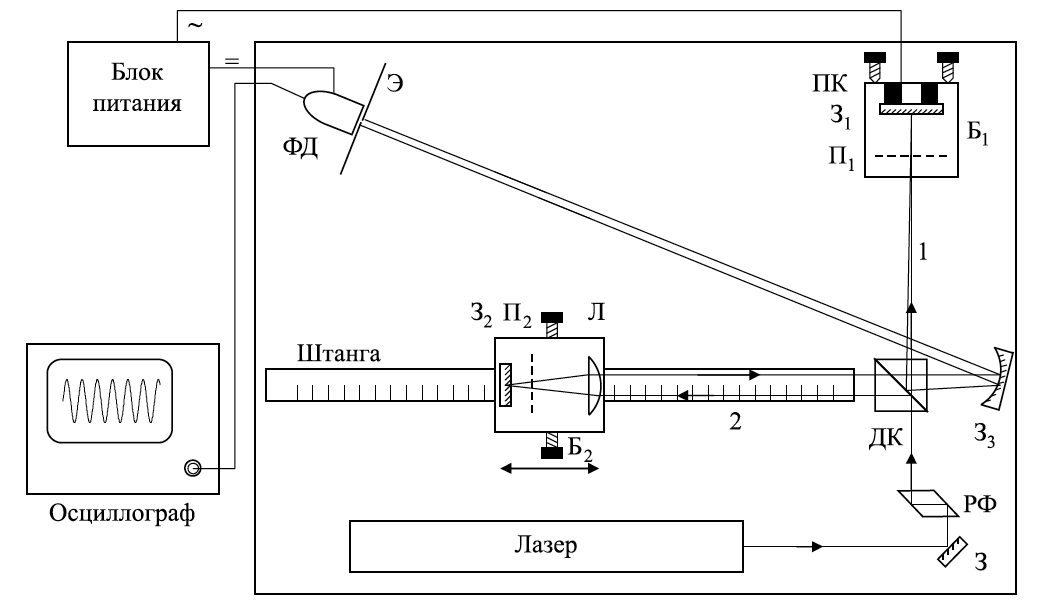
\includegraphics[width = 0.8\textwidth]{images/installation.png}
        \caption{Схема установки. З, $\text{З}_1$, $\text{З}_2$, $\text{З}_3$ -- зеркала; $\text{П}_1$, $\text{П}_2$ -- поляроиды; $\text{Б}_1$, $\text{Б}_2$ -- блоки № 1 и 2; ДК -- делительный кубик; РФ -- ромб Френеля; ФД -- фотодиод; Э -- экран; ПК -- пьезокерамика; Л -- линза.}
        \label{fig:installation_1}
    \end{figure}
    \end{frame}

    \begin{frame}{Фото экспериментальной установки}
    \small
    \begin{figure}[H]
        \centering
        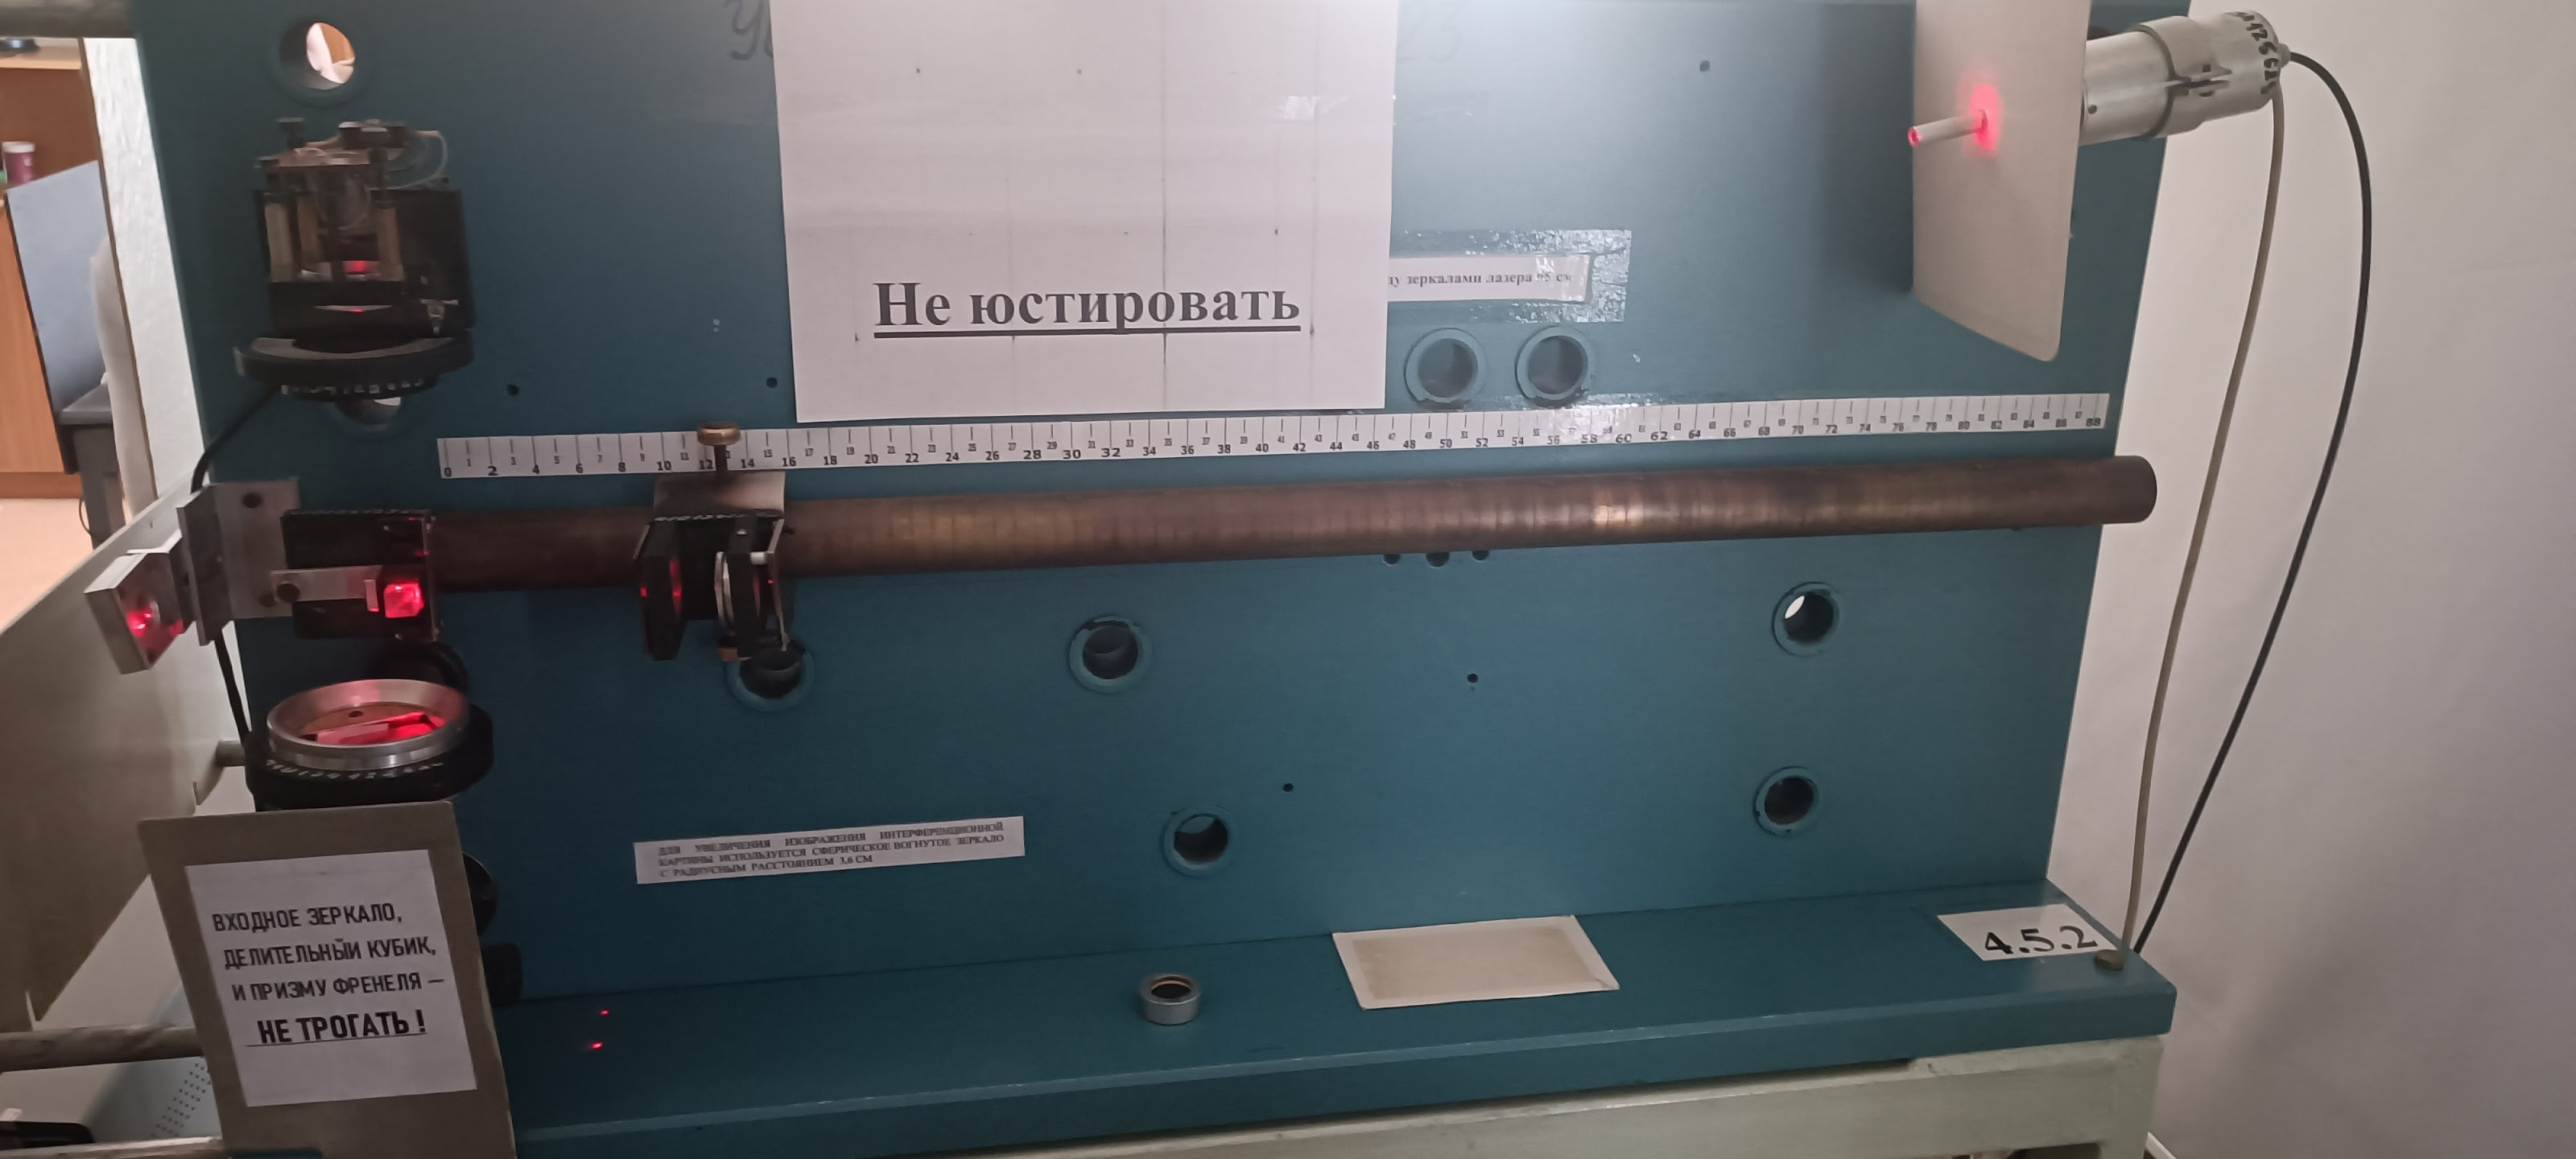
\includegraphics[width = \textwidth]{images/installation_photo.jpg}
        \caption{Фотография юстированной установки}
        \label{fig:installation_2}
    \end{figure}
    \end{frame}

    \begin{frame}{Измерение видности с помощью осциллографа}
    \begin{itemize}
        \item На осциллографе видны колебания из-за вибрирующей пьезокермики. Её длина меняется вследствие наличия на ней напряжение. Линия $0$ -- фоновая засветка, $h_1, h_2$ -- интенсивность света каждого из пучков, $h_3, h_4$ -- минимум и максимум интерференционной картины
        \begin{columns}[T]
            \begin{column}{0.5\textwidth}
                \centering
                \begin{figure}
                    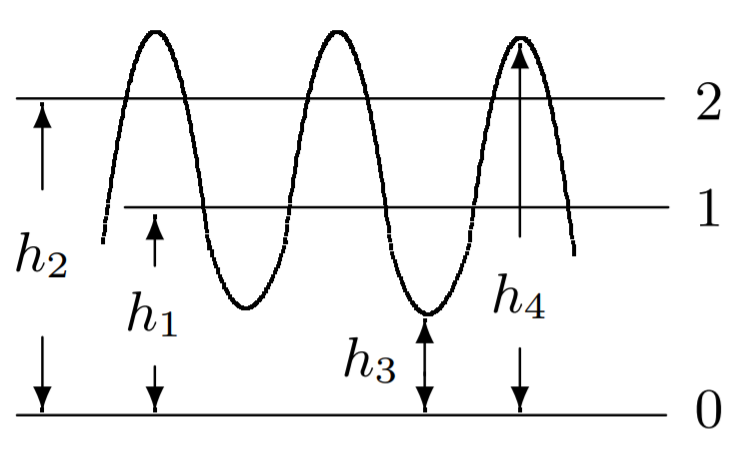
\includegraphics[width=\textwidth]{images/blabla.png}
                    \caption{Осциллограмма сигнала фотодиода}
                    \label{fig:osc}
                \end{figure}
            \end{column}
    
            \begin{column}{0.5\textwidth}
        
                \centering
                \small
                \begin{itemize}
                    \item Параметр $\delta$ для рассчёта $\gamma_1$:
                    \begin{equation}
                        \delta = \frac{h_1}{h_2}
                    \end{equation}
                    \item Видность интерференционной картины:
                    \begin{equation}
                        \gamma = \frac{h_4 - h_3}{h_4 + h_3}
                    \end{equation}
                \end{itemize}
                
            \end{column}%
        \end{columns}
    \end{itemize}
        
    \end{frame}
    
    \section{Измерения и обработка результатов} 
    
    \begin{frame}{Измерение видности от угла поворота поляроида}
        \begin{columns}
            \column{0.5\textwidth}
            \begin{figure}[H]
            \centering
                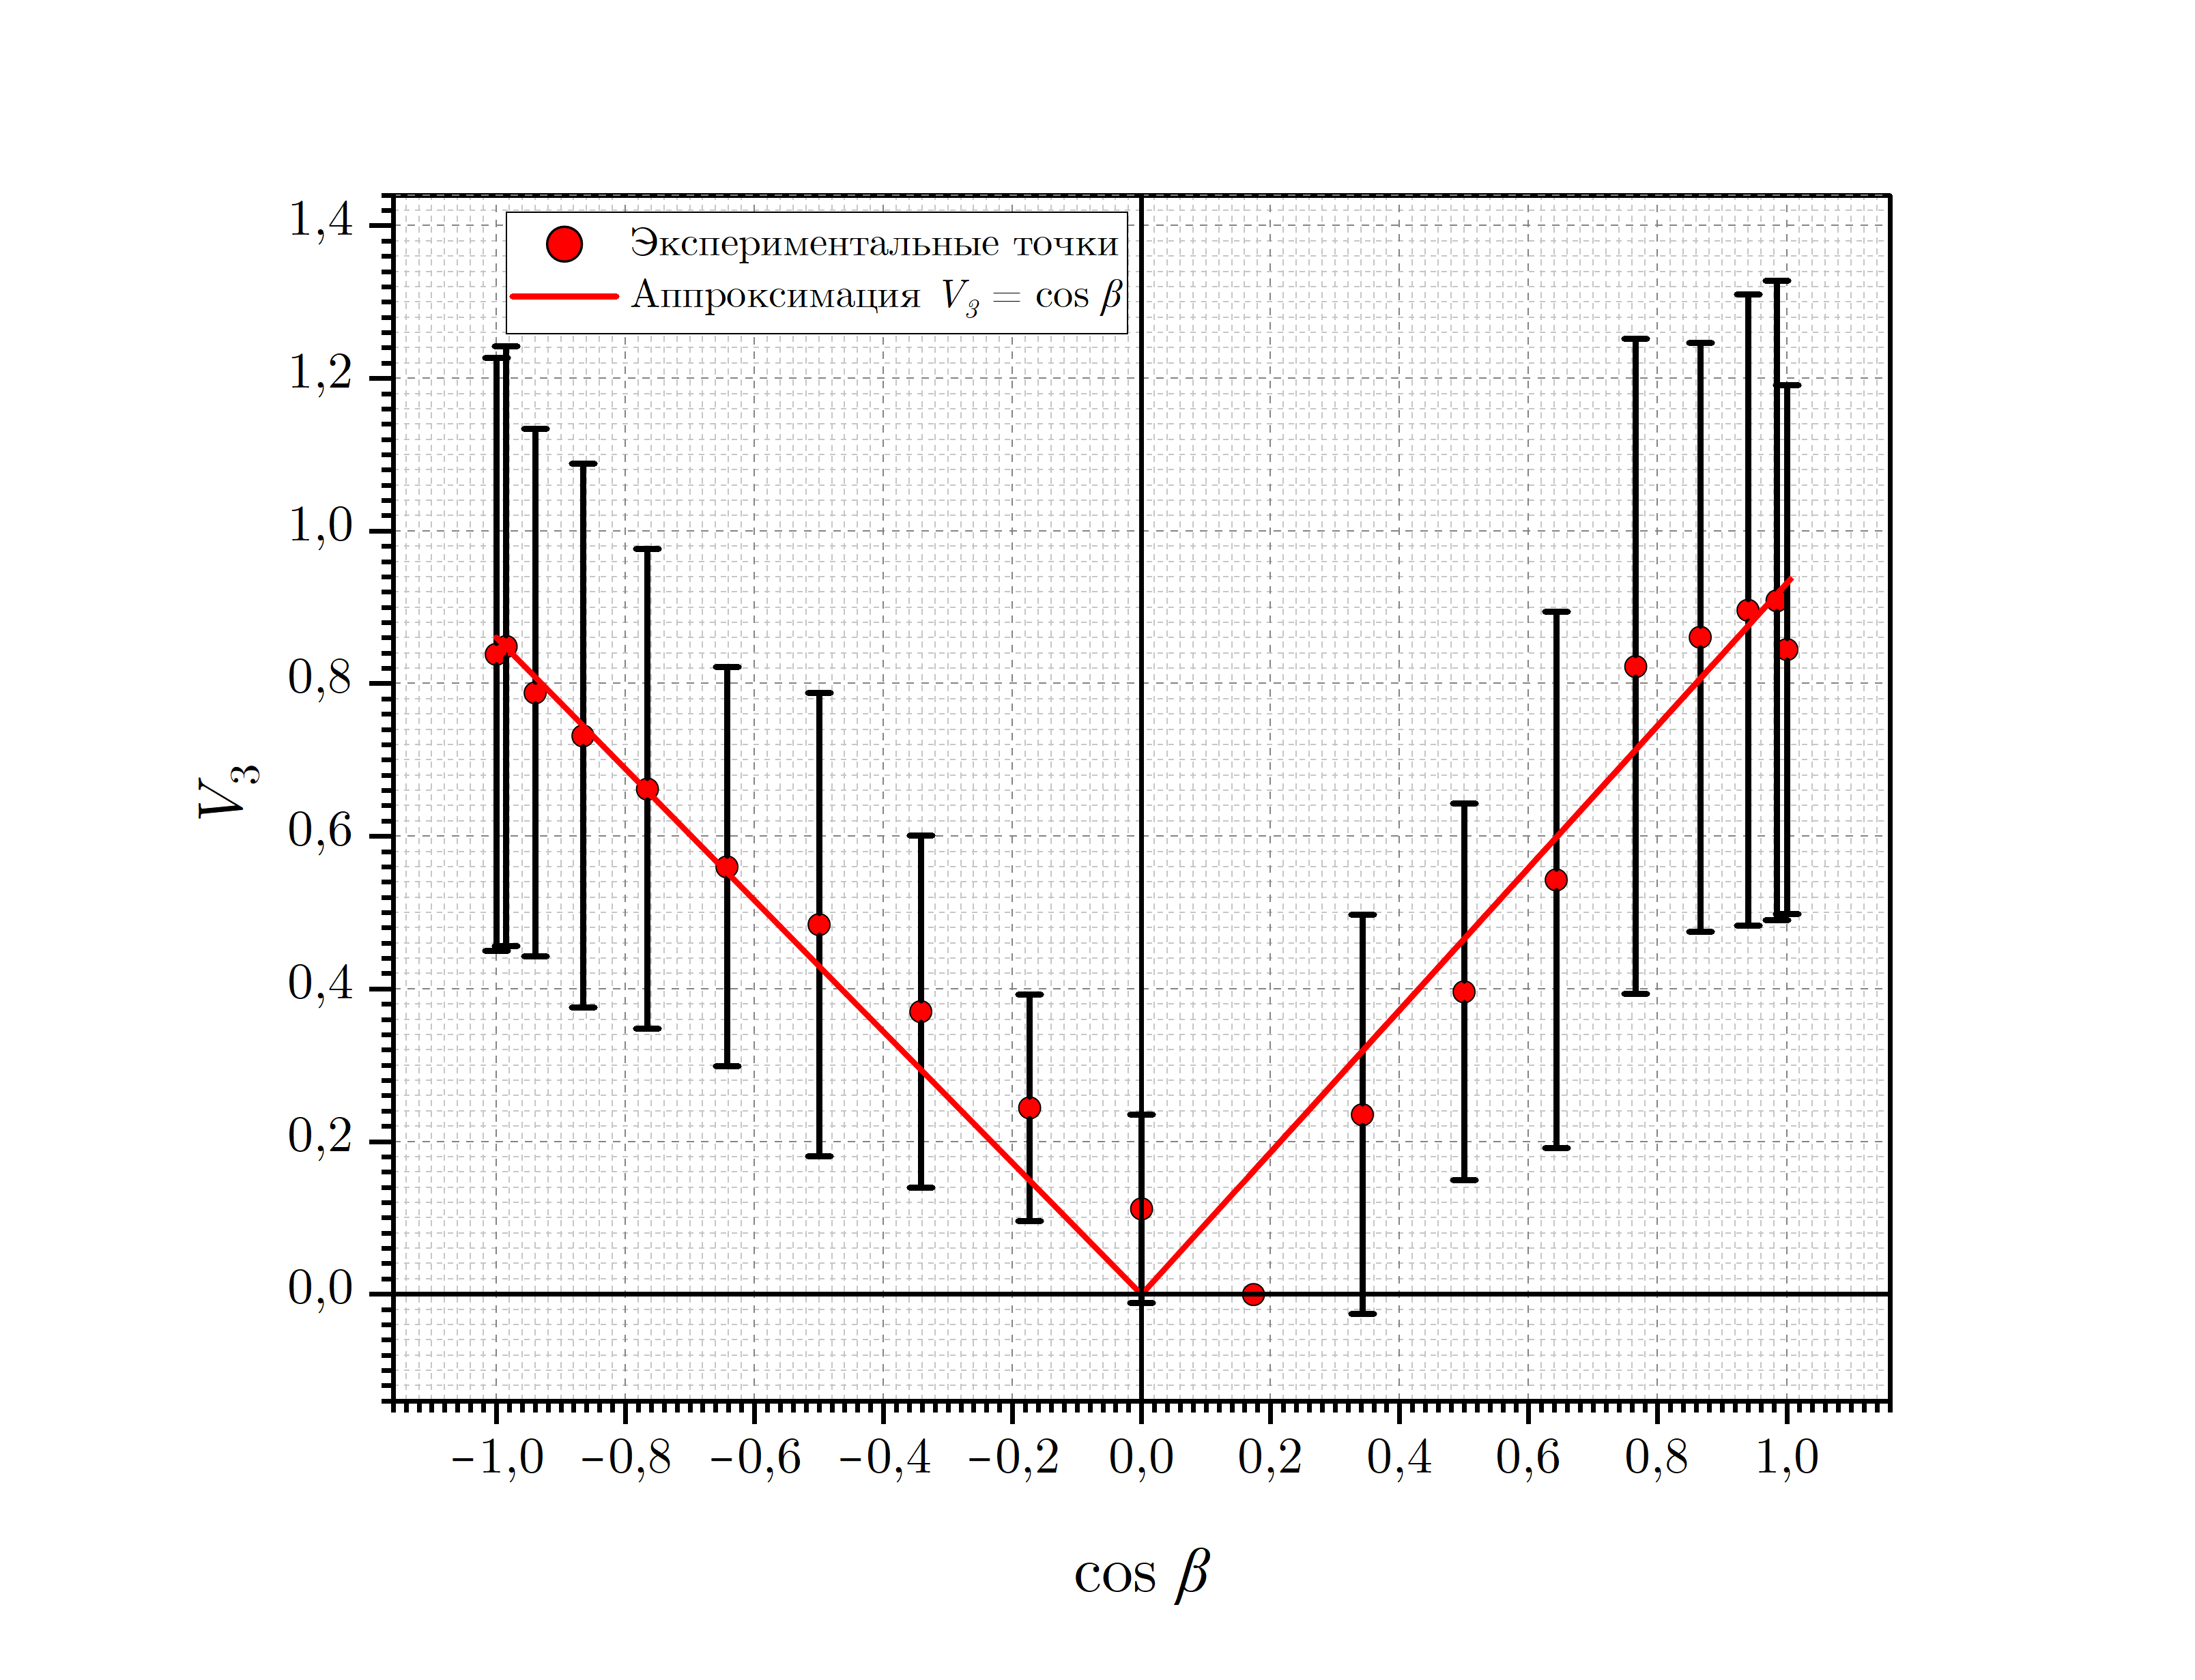
\includegraphics[width = \textwidth]{images/v3_cos.png}
                \caption{Зависимость $V_3 (\cos \beta )$}
            \end{figure}

            \column{0.5\textwidth}
            \begin{figure}[H]
            \centering
                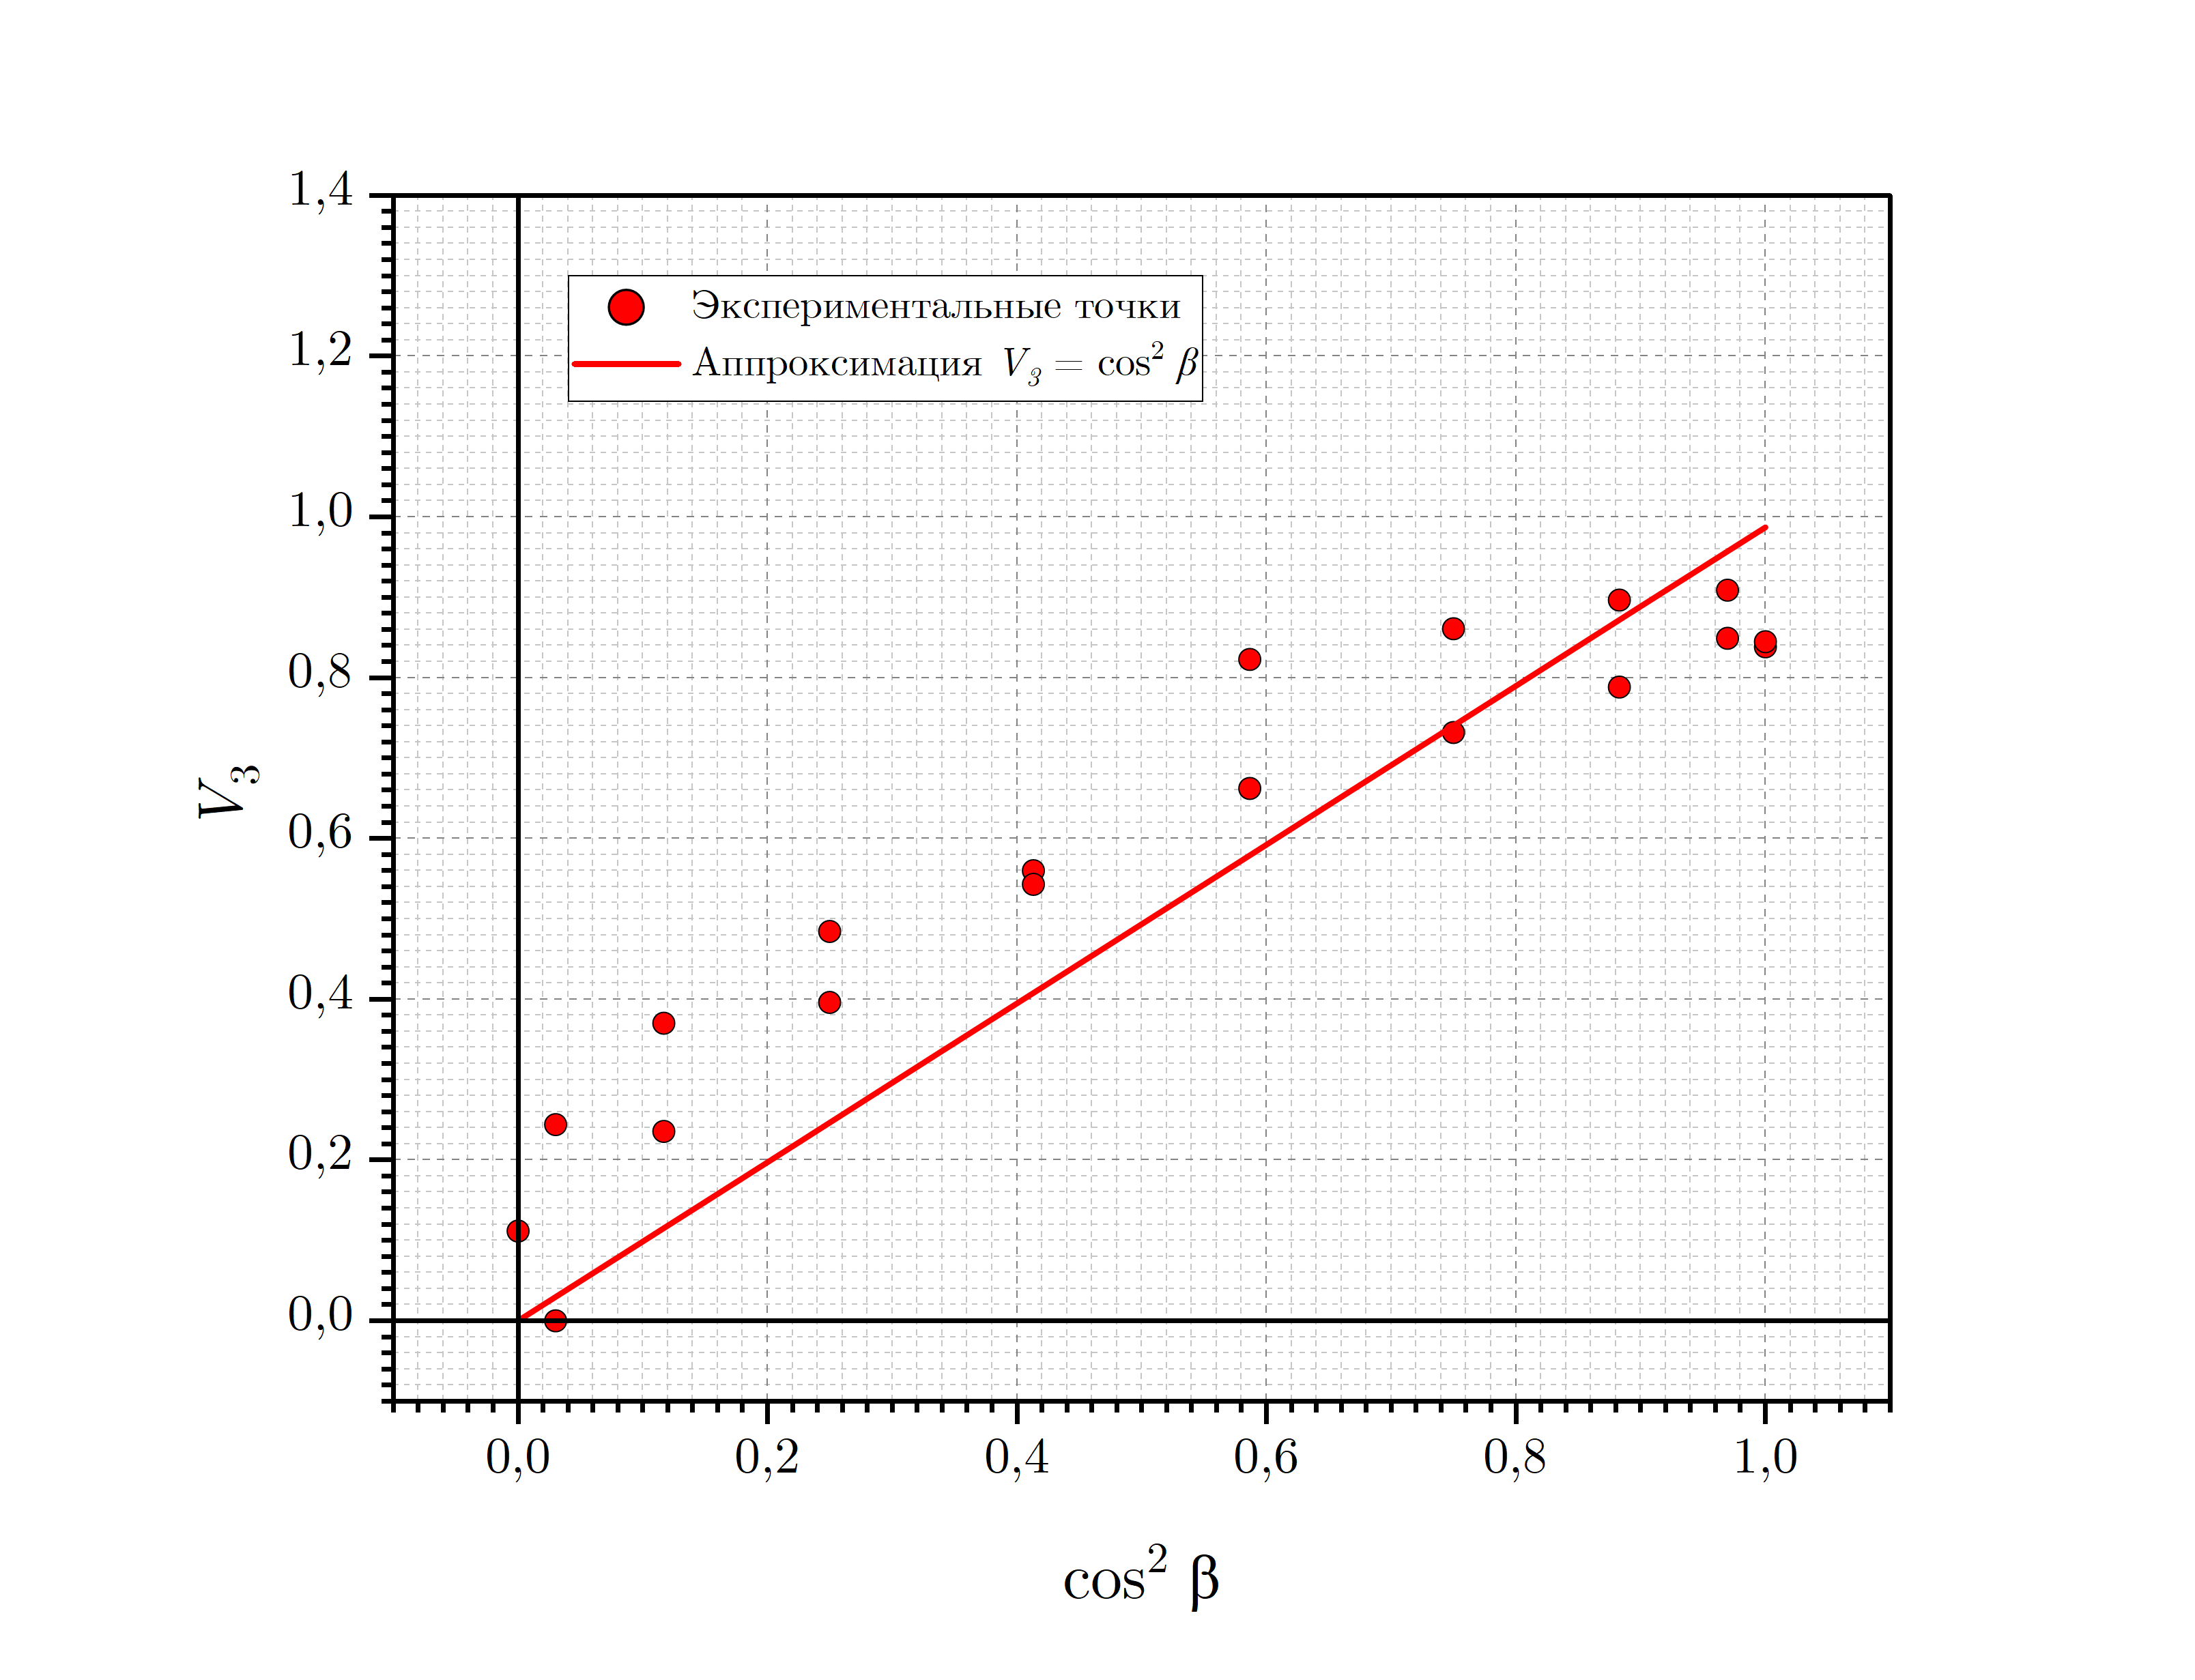
\includegraphics[width = 1.1\textwidth]{images/v3_coscos.png}
                \caption{Зависимость $V_3 (\cos^2 \beta )$}
            \end{figure}
        \end{columns}
    \end{frame}

    \begin{frame}{Измерение видности от угла поворота поляроида}
        \begin{columns}
            \column{0.5\textwidth}
            \begin{figure}[H]
            \centering
                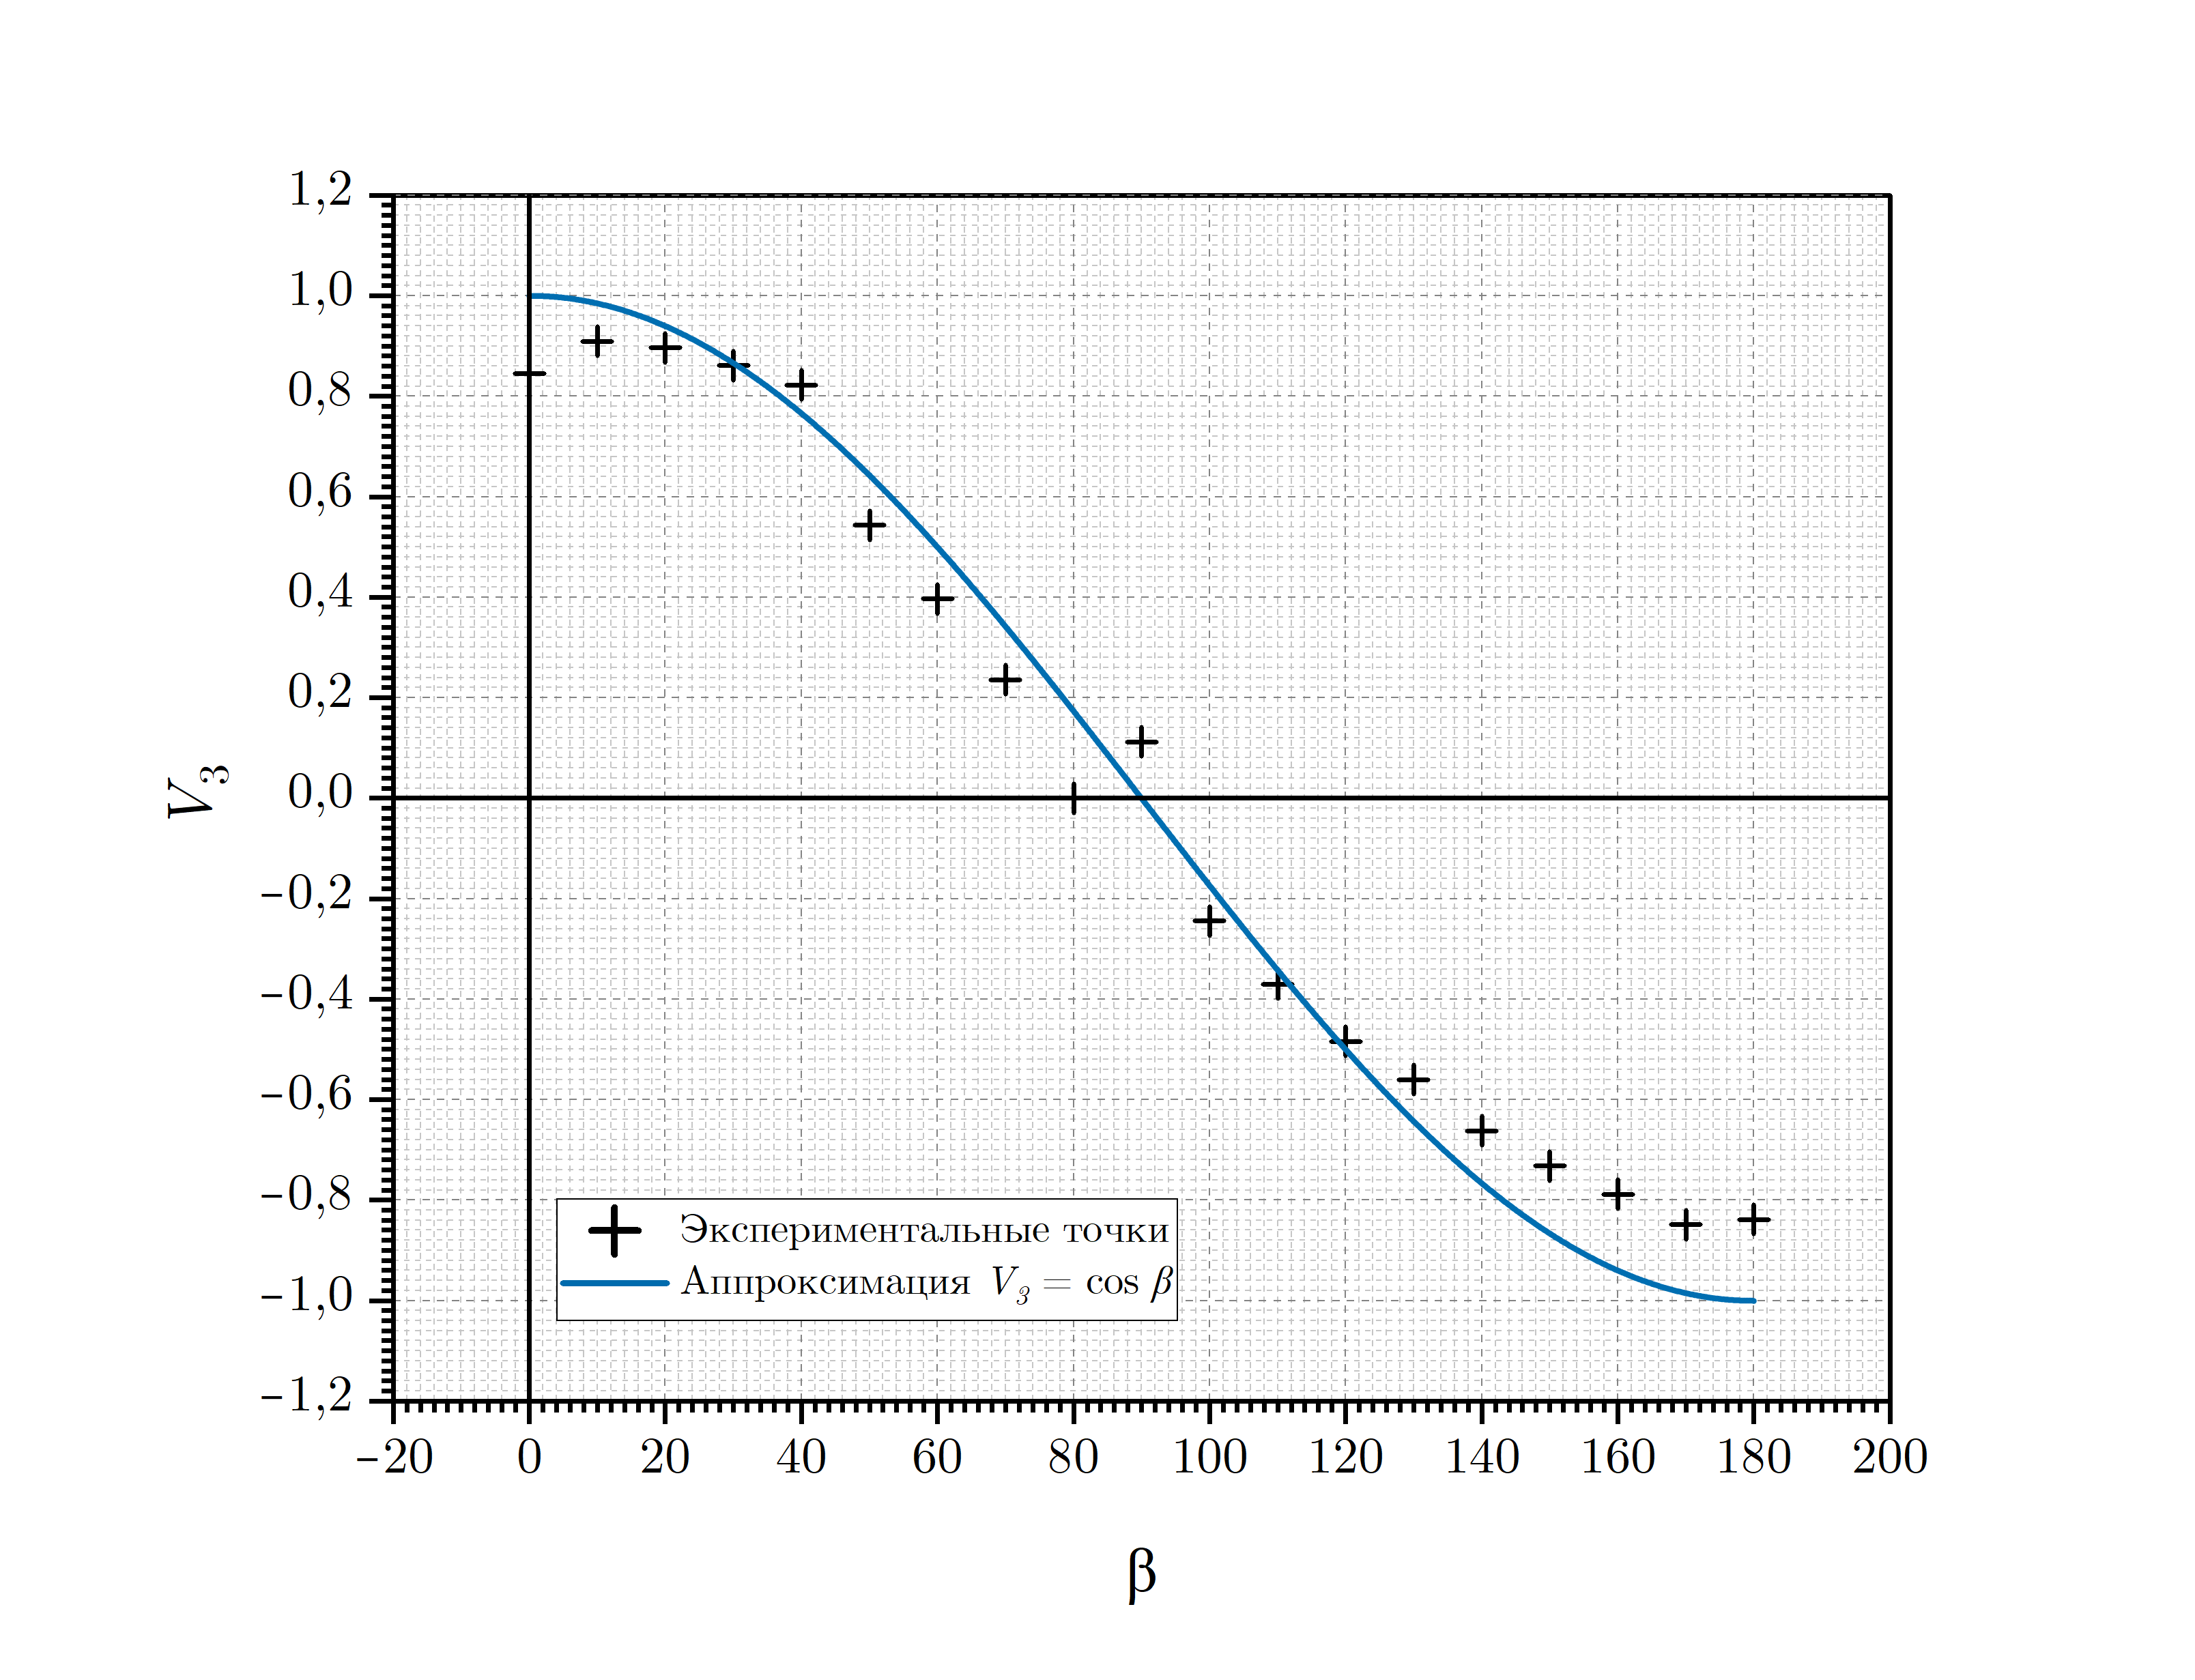
\includegraphics[width = \textwidth]{images/v3_cos_betta.png}
                \caption{Зависимость $V_3 = \cos \beta$}
            \end{figure}

            \column{0.5\textwidth}
            \begin{figure}[H]
            \centering
                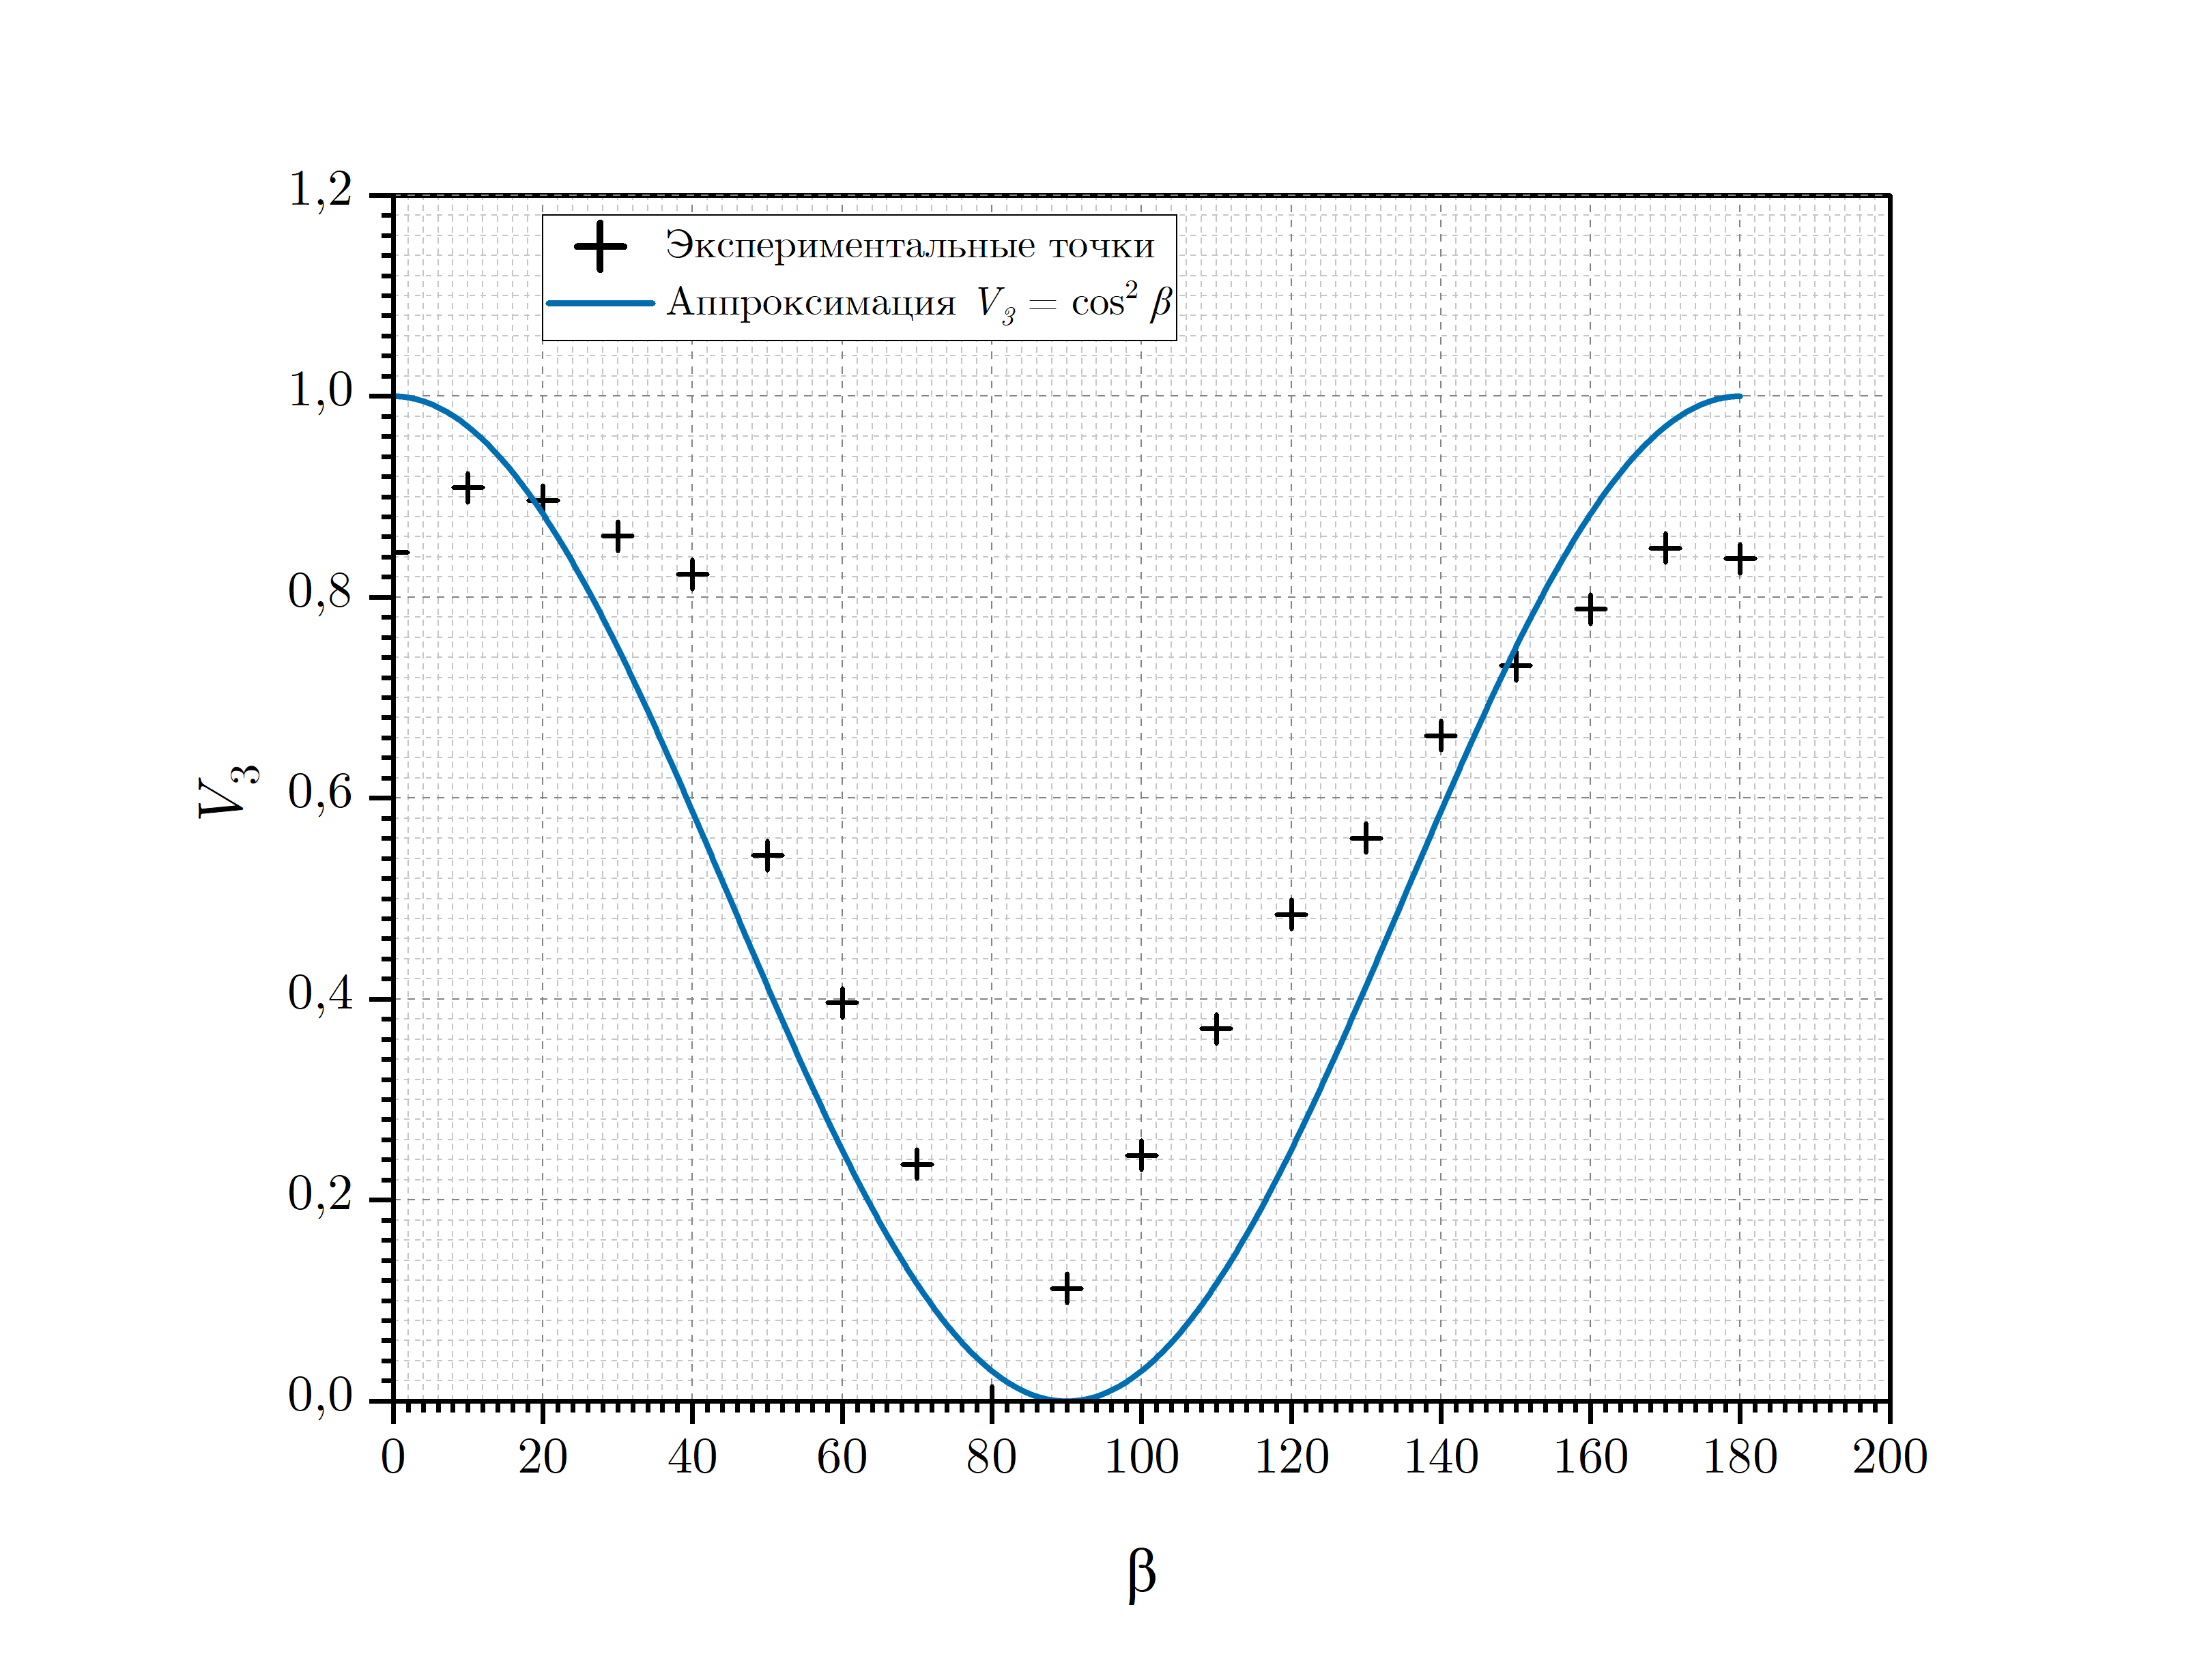
\includegraphics[width = \textwidth]{images/v3_coscos_betta.png}
                \caption{Зависимость $V_3 = \cos^2 \beta$}
            \end{figure}
        \end{columns}
    \end{frame}

    \begin{frame}{Анализ зависимости видности от угла поворота поляроида}
        \begin{itemize}
            \item Полученные данные лучше всего аппроксимировать функцией $V_3 = \cos \beta$
            \item Отсюда следует, что \textbf{поляризация -- линейная}, амплитуды волн не флуктуируют, а угол между плоскостями их поляризаций равен $\beta$
        \end{itemize}
    \end{frame}

    \begin{frame}{Измерение видности от дальности хода}
        \begin{columns}
            \column{0.5\textwidth}
            \begin{figure}[H]
            \centering
                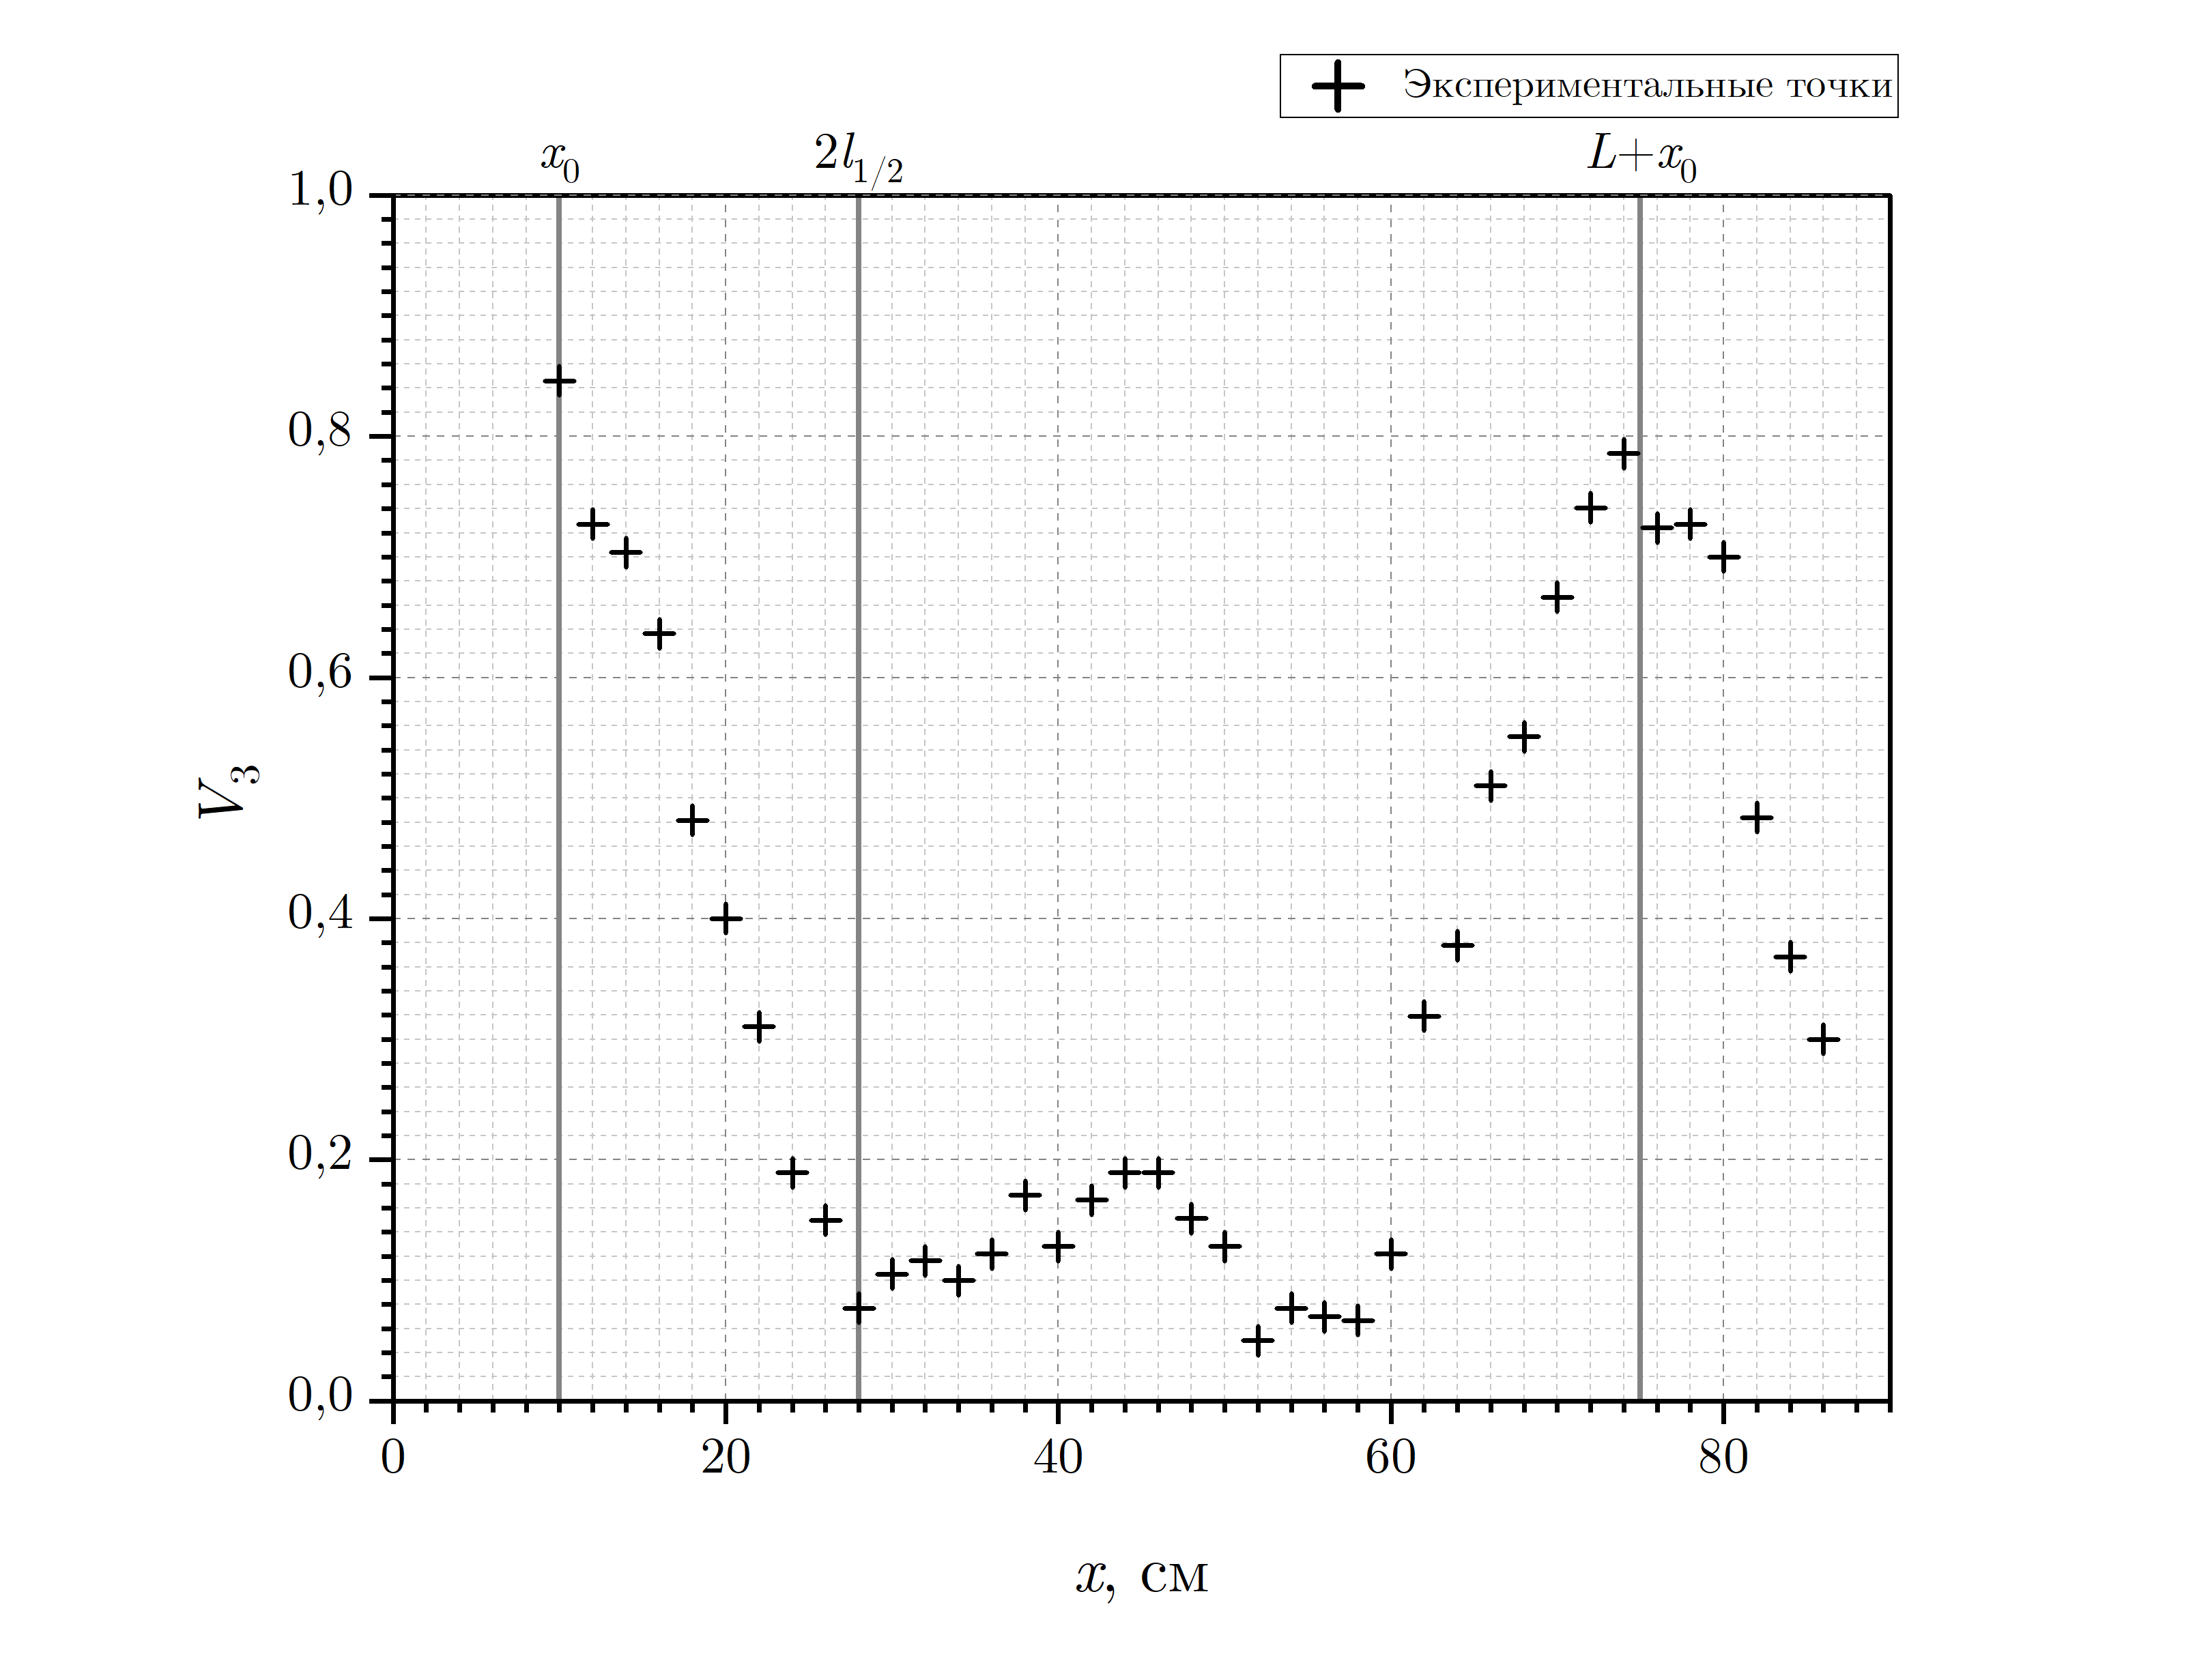
\includegraphics[width = \textwidth]{images/v2_x.png}
                \caption{Зависимость $V_2(x)$ от координаты блока $\text{Б}_2$}
            \end{figure}

            \column{0.5\textwidth}
            \begin{itemize}
                \item $L = \left( 65 \pm 2 \right) \text{ см}$ -- расстояние между зеркалами оптического резонатора лазера
                \item $\Delta \nu_m = \frac{c}{2L} \sim 2 \cdot 10^8 \text{ Гц}$ -- межмодовое расстояние
                \item $2l_{1/2} = \left( 28 \pm 2 \right) \text{ см}$ -- задержка на половине высоты главного максимума
                \item $\Delta F \approx 0.6 \frac{c}{l_{1/2}} = 10^{9} \text{ Гц}$ -- диапазон генерации продольных мод
                \item $n \approx 1 + 1.2 \frac{L}{l_{1/2}} \approx 7$ -- число мод
            \end{itemize}
            
        \end{columns}
    \end{frame}

\section{Заключение. Выводы}
    \begin{frame}{Заключение}
        \begin{itemize}
            \item В результате выполнения работы было исследовано влияние немонохроматичности света на видность интерференционной картины. Во время выполнения этой части работы было установлено, что поляризация излучения -- \textbf{линейная}
            \item Во второй части работы было найдено межмодовое расстояние $\Delta \nu_m = 2 \cdot 10^{8} \text{ Гц}$ ($\Delta \nu_{m}^{\text{табл}} = 10^{8} \text{ Гц}$) и число генерируемых лазером продольных мод $n \approx 7$ ($n^{\text{табл}} = 3-7$)
            \item Основной вклад в погрешность внесло измерение с помощью осциллографа интенсивности интерференционной картины и фоновой засветки
        \end{itemize}
    \end{frame}

    \section{Список литературы}
    \begin{frame}{Список литературы}
        \printbibliography
    \end{frame}
    
\end{document}